\documentclass[twoside]{book}

% Packages required by doxygen
\usepackage{fixltx2e}
\usepackage{calc}
\usepackage{doxygen}
\usepackage[export]{adjustbox} % also loads graphicx
\usepackage{graphicx}
\usepackage[utf8]{inputenc}
\usepackage{makeidx}
\usepackage{multicol}
\usepackage{multirow}
\PassOptionsToPackage{warn}{textcomp}
\usepackage{textcomp}
\usepackage[nointegrals]{wasysym}
\usepackage[table]{xcolor}

% Font selection
\usepackage[T1]{fontenc}
\usepackage[scaled=.90]{helvet}
\usepackage{courier}
\usepackage{amssymb}
\usepackage{sectsty}
\renewcommand{\familydefault}{\sfdefault}
\allsectionsfont{%
  \fontseries{bc}\selectfont%
  \color{darkgray}%
}
\renewcommand{\DoxyLabelFont}{%
  \fontseries{bc}\selectfont%
  \color{darkgray}%
}
\newcommand{\+}{\discretionary{\mbox{\scriptsize$\hookleftarrow$}}{}{}}

% Page & text layout
\usepackage{geometry}
\geometry{%
  a4paper,%
  top=2.5cm,%
  bottom=2.5cm,%
  left=2.5cm,%
  right=2.5cm%
}
\tolerance=750
\hfuzz=15pt
\hbadness=750
\setlength{\emergencystretch}{15pt}
\setlength{\parindent}{0cm}
\setlength{\parskip}{3ex plus 2ex minus 2ex}
\makeatletter
\renewcommand{\paragraph}{%
  \@startsection{paragraph}{4}{0ex}{-1.0ex}{1.0ex}{%
    \normalfont\normalsize\bfseries\SS@parafont%
  }%
}
\renewcommand{\subparagraph}{%
  \@startsection{subparagraph}{5}{0ex}{-1.0ex}{1.0ex}{%
    \normalfont\normalsize\bfseries\SS@subparafont%
  }%
}
\makeatother

% Headers & footers
\usepackage{fancyhdr}
\pagestyle{fancyplain}
\fancyhead[LE]{\fancyplain{}{\bfseries\thepage}}
\fancyhead[CE]{\fancyplain{}{}}
\fancyhead[RE]{\fancyplain{}{\bfseries\leftmark}}
\fancyhead[LO]{\fancyplain{}{\bfseries\rightmark}}
\fancyhead[CO]{\fancyplain{}{}}
\fancyhead[RO]{\fancyplain{}{\bfseries\thepage}}
\fancyfoot[LE]{\fancyplain{}{}}
\fancyfoot[CE]{\fancyplain{}{}}
\fancyfoot[RE]{\fancyplain{}{\bfseries\scriptsize Generated by Doxygen }}
\fancyfoot[LO]{\fancyplain{}{\bfseries\scriptsize Generated by Doxygen }}
\fancyfoot[CO]{\fancyplain{}{}}
\fancyfoot[RO]{\fancyplain{}{}}
\renewcommand{\footrulewidth}{0.4pt}
\renewcommand{\chaptermark}[1]{%
  \markboth{#1}{}%
}
\renewcommand{\sectionmark}[1]{%
  \markright{\thesection\ #1}%
}

% Indices & bibliography
\usepackage{natbib}
\usepackage[titles]{tocloft}
\setcounter{tocdepth}{3}
\setcounter{secnumdepth}{5}
\makeindex

% Hyperlinks (required, but should be loaded last)
\usepackage{ifpdf}
\ifpdf
  \usepackage[pdftex,pagebackref=true]{hyperref}
\else
  \usepackage[ps2pdf,pagebackref=true]{hyperref}
\fi
\hypersetup{%
  colorlinks=true,%
  linkcolor=blue,%
  citecolor=blue,%
  unicode%
}

% Custom commands
\newcommand{\clearemptydoublepage}{%
  \newpage{\pagestyle{empty}\cleardoublepage}%
}

\usepackage{caption}
\captionsetup{labelsep=space,justification=centering,font={bf},singlelinecheck=off,skip=4pt,position=top}

%===== C O N T E N T S =====

\begin{document}

% Titlepage & ToC
\hypersetup{pageanchor=false,
             bookmarksnumbered=true,
             pdfencoding=unicode
            }
\pagenumbering{roman}
\begin{titlepage}
\vspace*{7cm}
\begin{center}%
{\Large Mini\+S\+Hell }\\
\vspace*{1cm}
{\large Generated by Doxygen 1.8.11}\\
\end{center}
\end{titlepage}
\clearemptydoublepage
\tableofcontents
\clearemptydoublepage
\pagenumbering{arabic}
\hypersetup{pageanchor=true}

%--- Begin generated contents ---
\chapter{Mini\+S\+He\+LL}
\label{md_README}
\hypertarget{md_README}{}
P\+R\+O\+J\+ET \+: Mini\+S\+Hell « my\+\_\+sh » – à réaliser en binôme – Durée approximative $\sim$ 8h00min.

A l’aide des supports de cours et des mémentos et des exercices achevés en TP et du manuel Linux réalisez \+: (Tout code ou implémentation compilant ou non sera étudié, toute fois le barème sera adapté) Le présent sujet de projet comporte 3 pages

\subsection*{I – Synopsis}

L’objectif de ce projet et de réaliser -\/dans une proportion simplifiée-\/ l’implémentation d’un interpréteur de commande similaire à bash. Au lancement ce dernier doit pouvoir afficher un prompt attendant la saisie d’une commande ou d’un sous-\/ensemble de commandes.

Exemple \+: Prompt$>$ ls –a ; who Prompt$>$ ls –a $\vert$ grep toto Prompt$>$ date

\subsection*{II – Démarche}

Les commandes sont lancées par des processus fils laissant au père le rôle d’interpréteur. Ce dernier doit attendre la fin du/des processus fils pour afficher le résultat d’exécution du/des \hyperlink{structcommande}{commande(s)} soumises. Certaines commandes et variables devront être internes (fonctionnalités built-\/in), c’est-\/à-\/dire, directement prises en compte par le code. Ainsi on distinguera trois phases distinctes \+: \begin{DoxyVerb}L’évaluation de l’expression soumise à l’interpréteur.
L’exécution ordonnancée du sous-ensemble de commandes.
La soumission du résultat d’exécution.
\end{DoxyVerb}


\subsection*{I\+II – Résultats attendus}

Le livrable attendu pour ce projet se résume en un code source compilable et exécutable répondant d’une part aux fonctions métiers suivantes \+:


\begin{DoxyItemize}
\item F\+M01 – Le binaire est capable d’exécuter une commande simple (ie \+: ls –l ; ps ; who) ✓
\item F\+M02 – Le binaire est capable d’exécuter un sous-\/ensemble de plusieurs commandes de sorte à prendre en compte \+: ✓
\begin{DoxyItemize}
\item Les opérateurs de contrôle \+: \&\& et $\vert$$\vert$
\item Les redirections de flux simples \+: $\vert$, $>$, $<$, $>$$>$, $<$$<$
\item L’exécution en arrière-\/plan \+: \&
\end{DoxyItemize}
\item F\+M03 – L’exécution des commandes internes (fonctionnalités built-\/in) suivantes \+: ✓
\begin{DoxyItemize}
\item cd -\/ Permettant de se déplacer au sein d’une arborescence de fichier.
\item pwd – Affichant la valeur de la variable contenant le chemin du répertoire courant.
\item exit – Permettant de quitter l’interpréteur.
\item echo – Permettant d’afficher du texte sur la sortie standard.
\end{DoxyItemize}
\item F\+M04 -\/ La persistance des commandes saisie dans un fichier (historique) ✓
\end{DoxyItemize}

D’autres fonctionnalités optionnelles peuvent êtres implémentés \+:


\begin{DoxyItemize}
\item F\+O01 – La réalisation d’un mode batch (ie \+: ./my\+\_\+shell –c « ls –al $\vert$ grep toto ») $\sim$
\item F\+O02 – La création de variables d’environnement
\item F\+O03 – La prise en charge d’alias
\end{DoxyItemize}

Concernant les exigences techniques attendues, vous devez respecter les contraintes suivantes \+:


\begin{DoxyItemize}
\item C\+T01 – La compilation du projet doit se faire via un Makefile. ✓
\item C\+T02 – La définitions des structures doit se faire dans un fichier \hyperlink{typedef_8h}{typedef.\+h}. ✓
\item C\+T03 – La définition des méthodes protoype (.h) \& implémentation (.c) doit se faire de manière séparée autant que faire se peut. ✓
\item C\+T04 – Le code produit doit être documenté. $\sim$
\item C\+T05 – La gestion des erreurs doit se faire via « les mécanismes proposés par errno ». ✓
\end{DoxyItemize}

D’autres contraintes techniques peuvent être prises en compte \+:
\begin{DoxyItemize}
\item C\+T\+O01 – La documentation du code générée via l’utilitaire doxygen.
\item C\+T\+O02 – Le code est soumis à un contrôle de couverture via l’utilitaire gcov.
\item C\+T\+O03 – Une page de manuel Linux est rédigée pour détailler l’exécution du shell.
\end{DoxyItemize}

\subsection*{IV – Evaluation}

Ce projet est à réaliser en binôme et donnera lieu à une présentation d’environs 15min répartie en deux phases \+: présentation\&démonstration suivi d’un partie consacrée aux questions. (Un support de présentation pourra être utilisé mais ne devra pas contenir plus de 5 diapos).

La réalisation de ce shell simplifié vise à mettre en œuvre l’ensemble des connaissances abordées au cours de ce module. La restitution du plus grand nombre de notions à travers le code produit vous permet de valider vos compétences.

Ainsi la réalisation de l’ensemble des fonctionnalités métiers FM 1 à 4 ainsi que le respect des contraintes techniques vous assure une note supérieure à la moyenne signifiant l’acquis des connaissances. Toutefois la réalisation des fonctionnalités métiers et/ou optionnelles vous permettent d’augmenter votre note le cas échéant. 
\chapter{Class Index}
\section{Class List}
Here are the classes, structs, unions and interfaces with brief descriptions\+:\begin{DoxyCompactList}
\item\contentsline{section}{\hyperlink{structnode}{node} }{\pageref{structnode}}{}
\item\contentsline{section}{\hyperlink{structstackNode}{stack\+Node} \\*Structure noeud de pile contenant la donnee et le noeud suivant }{\pageref{structstackNode}}{}
\item\contentsline{section}{\hyperlink{structstackTree}{stack\+Tree} \\*Structure pile d\textquotesingle{}arbre contenant un arbre et l\textquotesingle{}arbre suivant }{\pageref{structstackTree}}{}
\item\contentsline{section}{\hyperlink{structtree}{tree} \\*Structure d\textquotesingle{}arbre binaire }{\pageref{structtree}}{}
\end{DoxyCompactList}

\chapter{File Index}
\section{File List}
Here is a list of all documented files with brief descriptions\+:\begin{DoxyCompactList}
\item\contentsline{section}{include/\hyperlink{builtin_8h}{builtin.\+h} \\*Fonctions du Shell }{\pageref{builtin_8h}}{}
\item\contentsline{section}{include/\hyperlink{parser_8h}{parser.\+h} \\*Gestion du Shell }{\pageref{parser_8h}}{}
\item\contentsline{section}{include/\hyperlink{shell_8h}{shell.\+h} \\*Gestion du Shell }{\pageref{shell_8h}}{}
\item\contentsline{section}{include/\hyperlink{stack_8h}{stack.\+h} \\*Pile contenant des strings (et on parle bien des chaînes de caractères ;)) }{\pageref{stack_8h}}{}
\item\contentsline{section}{include/\hyperlink{stackTree_8h}{stack\+Tree.\+h} \\*Pile contenant des arbres }{\pageref{stackTree_8h}}{}
\item\contentsline{section}{include/\hyperlink{tree_8h}{tree.\+h} \\*Gestion du Shell }{\pageref{tree_8h}}{}
\item\contentsline{section}{include/\hyperlink{typedef_8h}{typedef.\+h} \\*Définition des types }{\pageref{typedef_8h}}{}
\end{DoxyCompactList}

\chapter{Class Documentation}
\hypertarget{structcommand}{}\section{command Struct Reference}
\label{structcommand}\index{command@{command}}
\subsection*{Public Attributes}
\begin{DoxyCompactItemize}
\item 
const char $\ast$$\ast$ {\bfseries argv}\hypertarget{structcommand_a997f4f41a0e711df10c1cae633973bf2}{}\label{structcommand_a997f4f41a0e711df10c1cae633973bf2}

\end{DoxyCompactItemize}


The documentation for this struct was generated from the following file\+:\begin{DoxyCompactItemize}
\item 
include/\hyperlink{typedef_8h}{typedef.\+h}\end{DoxyCompactItemize}

\hypertarget{structcommande}{}\section{commande Struct Reference}
\label{structcommande}\index{commande@{commande}}


Structure des commandes, tableau de la commande et de ses arguments.  




{\ttfamily \#include $<$typedef.\+h$>$}



\subsection{Detailed Description}
Structure des commandes, tableau de la commande et de ses arguments. 

The documentation for this struct was generated from the following file\+:\begin{DoxyCompactItemize}
\item 
include/\hyperlink{typedef_8h}{typedef.\+h}\end{DoxyCompactItemize}

\hypertarget{structnode}{}\section{node Struct Reference}
\label{structnode}\index{node@{node}}


Collaboration diagram for node\+:\nopagebreak
\begin{figure}[H]
\begin{center}
\leavevmode
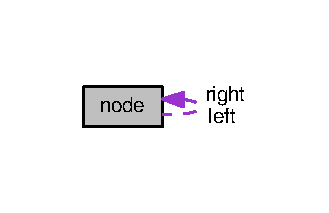
\includegraphics[width=158pt]{structnode__coll__graph}
\end{center}
\end{figure}
\subsection*{Public Attributes}
\begin{DoxyCompactItemize}
\item 
char $\ast$ {\bfseries value}\hypertarget{structnode_a0d2c1eb2a9662a891bb09807232d7f9f}{}\label{structnode_a0d2c1eb2a9662a891bb09807232d7f9f}

\item 
\hyperlink{structnode}{Tree} {\bfseries left}\hypertarget{structnode_a8bb8b7799bf138f227ce9d05ba8d3ca4}{}\label{structnode_a8bb8b7799bf138f227ce9d05ba8d3ca4}

\item 
\hyperlink{structnode}{Tree} {\bfseries right}\hypertarget{structnode_ade8fc5b5eff73152fc0b9c5c6ca6f0dd}{}\label{structnode_ade8fc5b5eff73152fc0b9c5c6ca6f0dd}

\end{DoxyCompactItemize}


The documentation for this struct was generated from the following file\+:\begin{DoxyCompactItemize}
\item 
include/\hyperlink{typedef_8h}{typedef.\+h}\end{DoxyCompactItemize}

\hypertarget{structstackNode}{}\section{stack\+Node Struct Reference}
\label{structstackNode}\index{stack\+Node@{stack\+Node}}


Structure noeud de pile contenant la donnee et le noeud suivant.  




{\ttfamily \#include $<$typedef.\+h$>$}



Collaboration diagram for stack\+Node\+:\nopagebreak
\begin{figure}[H]
\begin{center}
\leavevmode
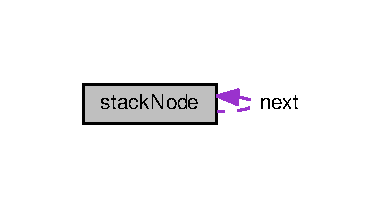
\includegraphics[width=184pt]{structstackNode__coll__graph}
\end{center}
\end{figure}
\subsection*{Public Attributes}
\begin{DoxyCompactItemize}
\item 
char $\ast$ {\bfseries data}\hypertarget{structstackNode_ab8a7f2b607f656ddbdaed84d1c5acbae}{}\label{structstackNode_ab8a7f2b607f656ddbdaed84d1c5acbae}

\item 
\hyperlink{structstackNode}{Stack} {\bfseries next}\hypertarget{structstackNode_a7225663fc2f1d3bad4623de65857c461}{}\label{structstackNode_a7225663fc2f1d3bad4623de65857c461}

\end{DoxyCompactItemize}


\subsection{Detailed Description}
Structure noeud de pile contenant la donnee et le noeud suivant. 

The documentation for this struct was generated from the following file\+:\begin{DoxyCompactItemize}
\item 
include/\hyperlink{typedef_8h}{typedef.\+h}\end{DoxyCompactItemize}

\hypertarget{structstackTree}{}\section{stack\+Tree Struct Reference}
\label{structstackTree}\index{stack\+Tree@{stack\+Tree}}


Collaboration diagram for stack\+Tree\+:\nopagebreak
\begin{figure}[H]
\begin{center}
\leavevmode
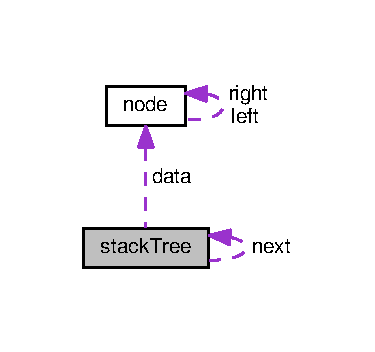
\includegraphics[width=180pt]{structstackTree__coll__graph}
\end{center}
\end{figure}
\subsection*{Public Attributes}
\begin{DoxyCompactItemize}
\item 
\hyperlink{structnode}{Tree} {\bfseries data}\hypertarget{structstackTree_a0948f3bec59d376fcb496088ef1eb390}{}\label{structstackTree_a0948f3bec59d376fcb496088ef1eb390}

\item 
\hyperlink{structstackTree}{Stack\+Tree} {\bfseries next}\hypertarget{structstackTree_ab01d5af00bf143c04cdb6c03ff3b4fb5}{}\label{structstackTree_ab01d5af00bf143c04cdb6c03ff3b4fb5}

\end{DoxyCompactItemize}


The documentation for this struct was generated from the following file\+:\begin{DoxyCompactItemize}
\item 
include/\hyperlink{typedef_8h}{typedef.\+h}\end{DoxyCompactItemize}

\hypertarget{structtree}{}\section{tree Struct Reference}
\label{structtree}\index{tree@{tree}}


Structure d\textquotesingle{}arbre binaire.  




{\ttfamily \#include $<$typedef.\+h$>$}



\subsection{Detailed Description}
Structure d\textquotesingle{}arbre binaire. 

The documentation for this struct was generated from the following file\+:\begin{DoxyCompactItemize}
\item 
include/\hyperlink{typedef_8h}{typedef.\+h}\end{DoxyCompactItemize}

\chapter{File Documentation}
\hypertarget{builtin_8h}{}\section{include/builtin.h File Reference}
\label{builtin_8h}\index{include/builtin.\+h@{include/builtin.\+h}}


Fonctions du Shell.  


{\ttfamily \#include \char`\"{}typedef.\+h\char`\"{}}\\*
Include dependency graph for builtin.\+h\+:\nopagebreak
\begin{figure}[H]
\begin{center}
\leavevmode
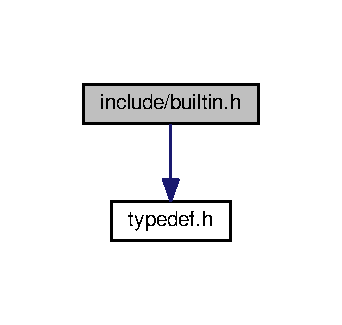
\includegraphics[width=164pt]{builtin_8h__incl}
\end{center}
\end{figure}
\subsection*{Functions}
\begin{DoxyCompactItemize}
\item 
void \hyperlink{builtin_8h_ac2badb93ccbe02d9462229285fc0184b}{cd\+Cmd} (char $\ast$$\ast$arg)
\begin{DoxyCompactList}\small\item\em Reproduit la commande \char`\"{}cd\char`\"{}. \end{DoxyCompactList}\item 
void \hyperlink{builtin_8h_a7363ac1891ce8f70c4c548aaebb16d24}{pwd\+Cmd} ()
\begin{DoxyCompactList}\small\item\em Reproduit la commande \char`\"{}pwd\char`\"{}. \end{DoxyCompactList}\item 
void \hyperlink{builtin_8h_ac9aab741f67d8c4ed42dff107e1cabdd}{exit\+Cmd} ()\hypertarget{builtin_8h_ac9aab741f67d8c4ed42dff107e1cabdd}{}\label{builtin_8h_ac9aab741f67d8c4ed42dff107e1cabdd}

\begin{DoxyCompactList}\small\item\em Quitte le processus courant. \end{DoxyCompactList}\item 
void \hyperlink{builtin_8h_ab2a46d03e0f6275654d6afdb4b092283}{echo\+Cmd} (char $\ast$$\ast$arg)
\begin{DoxyCompactList}\small\item\em Reproduit la commande \char`\"{}echo\char`\"{}. \end{DoxyCompactList}\end{DoxyCompactItemize}


\subsection{Detailed Description}
Fonctions du Shell. 

\begin{DoxyAuthor}{Author}
Loïc.\+B et Jean.\+S
\end{DoxyAuthor}
Reproduction des fonctions du Shell 

\subsection{Function Documentation}
\index{builtin.\+h@{builtin.\+h}!cd\+Cmd@{cd\+Cmd}}
\index{cd\+Cmd@{cd\+Cmd}!builtin.\+h@{builtin.\+h}}
\subsubsection[{\texorpdfstring{cd\+Cmd(char $\ast$$\ast$arg)}{cdCmd(char **arg)}}]{\setlength{\rightskip}{0pt plus 5cm}char $\ast$ cd\+Cmd (
\begin{DoxyParamCaption}
\item[{char $\ast$$\ast$}]{arg}
\end{DoxyParamCaption}
)}\hypertarget{builtin_8h_ac2badb93ccbe02d9462229285fc0184b}{}\label{builtin_8h_ac2badb93ccbe02d9462229285fc0184b}


Reproduit la commande \char`\"{}cd\char`\"{}. 


\begin{DoxyParams}{Parameters}
{\em Chemin} & du répertoire cible \\
\hline
\end{DoxyParams}
\begin{DoxyReturn}{Returns}
Chemin du répertoire cible 
\end{DoxyReturn}
\index{builtin.\+h@{builtin.\+h}!echo\+Cmd@{echo\+Cmd}}
\index{echo\+Cmd@{echo\+Cmd}!builtin.\+h@{builtin.\+h}}
\subsubsection[{\texorpdfstring{echo\+Cmd(char $\ast$$\ast$arg)}{echoCmd(char **arg)}}]{\setlength{\rightskip}{0pt plus 5cm}void echo\+Cmd (
\begin{DoxyParamCaption}
\item[{char $\ast$$\ast$}]{arg}
\end{DoxyParamCaption}
)}\hypertarget{builtin_8h_ab2a46d03e0f6275654d6afdb4b092283}{}\label{builtin_8h_ab2a46d03e0f6275654d6afdb4b092283}


Reproduit la commande \char`\"{}echo\char`\"{}. 


\begin{DoxyParams}{Parameters}
{\em Chaîne} & à afficher \\
\hline
\end{DoxyParams}
\begin{DoxyReturn}{Returns}
Chaîne à afficher 
\end{DoxyReturn}
\index{builtin.\+h@{builtin.\+h}!pwd\+Cmd@{pwd\+Cmd}}
\index{pwd\+Cmd@{pwd\+Cmd}!builtin.\+h@{builtin.\+h}}
\subsubsection[{\texorpdfstring{pwd\+Cmd()}{pwdCmd()}}]{\setlength{\rightskip}{0pt plus 5cm}void pwd\+Cmd (
\begin{DoxyParamCaption}
{}
\end{DoxyParamCaption}
)}\hypertarget{builtin_8h_a7363ac1891ce8f70c4c548aaebb16d24}{}\label{builtin_8h_a7363ac1891ce8f70c4c548aaebb16d24}


Reproduit la commande \char`\"{}pwd\char`\"{}. 

\begin{DoxyReturn}{Returns}
Chemin du répertoire courant 
\end{DoxyReturn}

\hypertarget{typedef_8h}{}\section{include/typedef.h File Reference}
\label{typedef_8h}\index{include/typedef.\+h@{include/typedef.\+h}}


Définition des types.  


This graph shows which files directly or indirectly include this file\+:\nopagebreak
\begin{figure}[H]
\begin{center}
\leavevmode
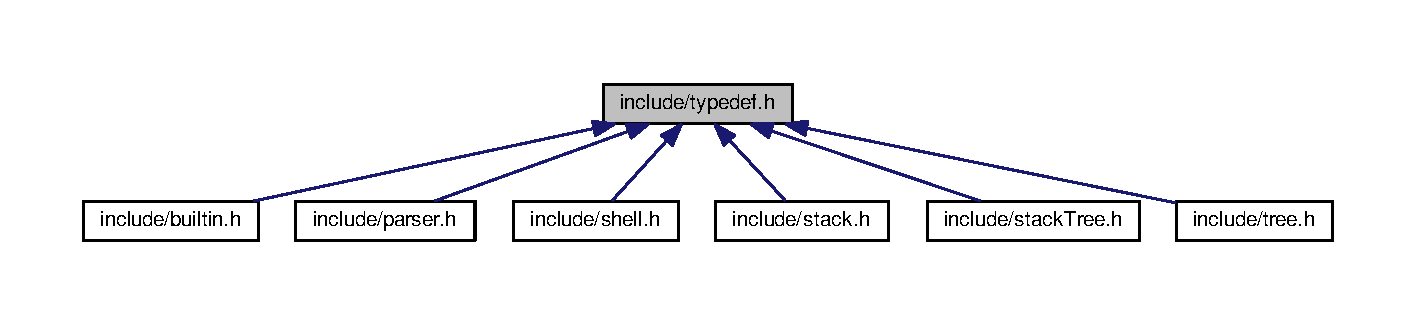
\includegraphics[width=350pt]{typedef_8h__dep__incl}
\end{center}
\end{figure}
\subsection*{Classes}
\begin{DoxyCompactItemize}
\item 
struct \hyperlink{structnode}{node}
\item 
struct \hyperlink{structstackNode}{stack\+Node}
\begin{DoxyCompactList}\small\item\em Structure noeud de pile contenant la donnee et le noeud suivant. \end{DoxyCompactList}\item 
struct \hyperlink{structstackTree}{stack\+Tree}
\begin{DoxyCompactList}\small\item\em Structure pile d\textquotesingle{}arbre contenant un arbre et l\textquotesingle{}arbre suivant. \end{DoxyCompactList}\end{DoxyCompactItemize}
\subsection*{Macros}
\begin{DoxyCompactItemize}
\item 
\#define \hyperlink{typedef_8h_af1abcb51a4aa27a5a5a7958c03448134}{M\+A\+X\+\_\+\+C\+O\+M\+M\+A\+N\+D\+\_\+\+L\+E\+N\+G\+TH}~150
\item 
\#define {\bfseries M\+A\+X\+\_\+\+N\+U\+M\+B\+E\+R\+\_\+\+O\+F\+\_\+\+P\+A\+R\+A\+MS}~30\hypertarget{typedef_8h_a093500fedd419f3091cfb430da6165a0}{}\label{typedef_8h_a093500fedd419f3091cfb430da6165a0}

\item 
\#define {\bfseries M\+A\+X\+\_\+\+N\+U\+M\+B\+E\+R\+\_\+\+O\+F\+\_\+\+C\+MD}~30\hypertarget{typedef_8h_a93d1e42f20aca136db885b3ac86c2a18}{}\label{typedef_8h_a93d1e42f20aca136db885b3ac86c2a18}

\item 
\#define {\bfseries S\+T\+D\+IN}~0\hypertarget{typedef_8h_ac00bfb46347d26fdc58568fe1ab5fa5b}{}\label{typedef_8h_ac00bfb46347d26fdc58568fe1ab5fa5b}

\item 
\#define {\bfseries S\+T\+D\+O\+UT}~1\hypertarget{typedef_8h_a8875037d0772a4fc34516f1e03d7e238}{}\label{typedef_8h_a8875037d0772a4fc34516f1e03d7e238}

\item 
\#define {\bfseries S\+T\+D\+E\+RR}~2\hypertarget{typedef_8h_a3a540e3eef339eec06aff31c4ba1eb25}{}\label{typedef_8h_a3a540e3eef339eec06aff31c4ba1eb25}

\item 
\#define {\bfseries K\+N\+RM}~\char`\"{}\textbackslash{}x1B\mbox{[}0m\char`\"{}\hypertarget{typedef_8h_a137aa83ec74421d226a90c92ec032ac9}{}\label{typedef_8h_a137aa83ec74421d226a90c92ec032ac9}

\item 
\#define {\bfseries K\+R\+ED}~\char`\"{}\textbackslash{}x1B\mbox{[}31m\char`\"{}\hypertarget{typedef_8h_a66290957baed5df3930ada4cb8caccf1}{}\label{typedef_8h_a66290957baed5df3930ada4cb8caccf1}

\item 
\#define {\bfseries K\+G\+RN}~\char`\"{}\textbackslash{}x1B\mbox{[}32m\char`\"{}\hypertarget{typedef_8h_ac081c83b067273757f7a2e54a5957d41}{}\label{typedef_8h_ac081c83b067273757f7a2e54a5957d41}

\item 
\#define {\bfseries K\+Y\+EL}~\char`\"{}\textbackslash{}x1B\mbox{[}33m\char`\"{}\hypertarget{typedef_8h_a897b10d246533c95ba86cb79f92e465a}{}\label{typedef_8h_a897b10d246533c95ba86cb79f92e465a}

\item 
\#define {\bfseries K\+B\+LU}~\char`\"{}\textbackslash{}x1B\mbox{[}34m\char`\"{}\hypertarget{typedef_8h_a3f838f2fc3a9a3b434be606fc908964b}{}\label{typedef_8h_a3f838f2fc3a9a3b434be606fc908964b}

\item 
\#define {\bfseries K\+M\+AG}~\char`\"{}\textbackslash{}x1B\mbox{[}35m\char`\"{}\hypertarget{typedef_8h_a6825f05d3b9d619d91d79d0ef18bb8b2}{}\label{typedef_8h_a6825f05d3b9d619d91d79d0ef18bb8b2}

\item 
\#define {\bfseries K\+C\+YN}~\char`\"{}\textbackslash{}x1B\mbox{[}36m\char`\"{}\hypertarget{typedef_8h_a32036c94dbb166a3f874b7efc169841f}{}\label{typedef_8h_a32036c94dbb166a3f874b7efc169841f}

\item 
\#define {\bfseries K\+W\+HT}~\char`\"{}\textbackslash{}x1B\mbox{[}37m\char`\"{}\hypertarget{typedef_8h_af0036c8022c9980079ab17e5c87fd478}{}\label{typedef_8h_af0036c8022c9980079ab17e5c87fd478}

\item 
\#define {\bfseries B\+O\+LD}~\char`\"{}\textbackslash{}x1B\mbox{[}1m\char`\"{}\hypertarget{typedef_8h_a26cdbb1a00213c810caccf21cd33a631}{}\label{typedef_8h_a26cdbb1a00213c810caccf21cd33a631}

\end{DoxyCompactItemize}
\subsection*{Typedefs}
\begin{DoxyCompactItemize}
\item 
typedef struct \hyperlink{structnode}{node} $\ast$ {\bfseries Tree}\hypertarget{typedef_8h_a65cc6ee99f44c5fe2972d8ee7d895f68}{}\label{typedef_8h_a65cc6ee99f44c5fe2972d8ee7d895f68}

\item 
typedef struct \hyperlink{structstackNode}{stack\+Node} $\ast$ {\bfseries Stack}\hypertarget{typedef_8h_ad0aa4d116a878fdd7dcc9c82b4cb5446}{}\label{typedef_8h_ad0aa4d116a878fdd7dcc9c82b4cb5446}

\item 
typedef struct \hyperlink{structstackTree}{stack\+Tree} $\ast$ {\bfseries Stack\+Tree}\hypertarget{typedef_8h_a096a0a245198f21b66ce18ce1511fa23}{}\label{typedef_8h_a096a0a245198f21b66ce18ce1511fa23}

\end{DoxyCompactItemize}
\subsection*{Enumerations}
\begin{DoxyCompactItemize}
\item 
enum \hyperlink{typedef_8h_af6a258d8f3ee5206d682d799316314b1}{bool} \{ {\bfseries true}, 
{\bfseries false}
 \}\hypertarget{typedef_8h_af6a258d8f3ee5206d682d799316314b1}{}\label{typedef_8h_af6a258d8f3ee5206d682d799316314b1}
\begin{DoxyCompactList}\small\item\em Booléen. \end{DoxyCompactList}
\end{DoxyCompactItemize}


\subsection{Detailed Description}
Définition des types. 

\begin{DoxyAuthor}{Author}
Loïc.\+B et Jean.\+S
\end{DoxyAuthor}
Définitions des types 

\subsection{Macro Definition Documentation}
\index{typedef.\+h@{typedef.\+h}!M\+A\+X\+\_\+\+C\+O\+M\+M\+A\+N\+D\+\_\+\+L\+E\+N\+G\+TH@{M\+A\+X\+\_\+\+C\+O\+M\+M\+A\+N\+D\+\_\+\+L\+E\+N\+G\+TH}}
\index{M\+A\+X\+\_\+\+C\+O\+M\+M\+A\+N\+D\+\_\+\+L\+E\+N\+G\+TH@{M\+A\+X\+\_\+\+C\+O\+M\+M\+A\+N\+D\+\_\+\+L\+E\+N\+G\+TH}!typedef.\+h@{typedef.\+h}}
\subsubsection[{\texorpdfstring{M\+A\+X\+\_\+\+C\+O\+M\+M\+A\+N\+D\+\_\+\+L\+E\+N\+G\+TH}{MAX_COMMAND_LENGTH}}]{\setlength{\rightskip}{0pt plus 5cm}\#define M\+A\+X\+\_\+\+C\+O\+M\+M\+A\+N\+D\+\_\+\+L\+E\+N\+G\+TH~150}\hypertarget{typedef_8h_af1abcb51a4aa27a5a5a7958c03448134}{}\label{typedef_8h_af1abcb51a4aa27a5a5a7958c03448134}
Variable globale, gere la taille des differents tableaux du shell 
%--- End generated contents ---

% Index
\backmatter
\newpage
\phantomsection
\clearemptydoublepage
\addcontentsline{toc}{chapter}{Index}
\printindex

\end{document}
